\section{LLM whiteboard}

\begin{figure}[!h]
    \centering
    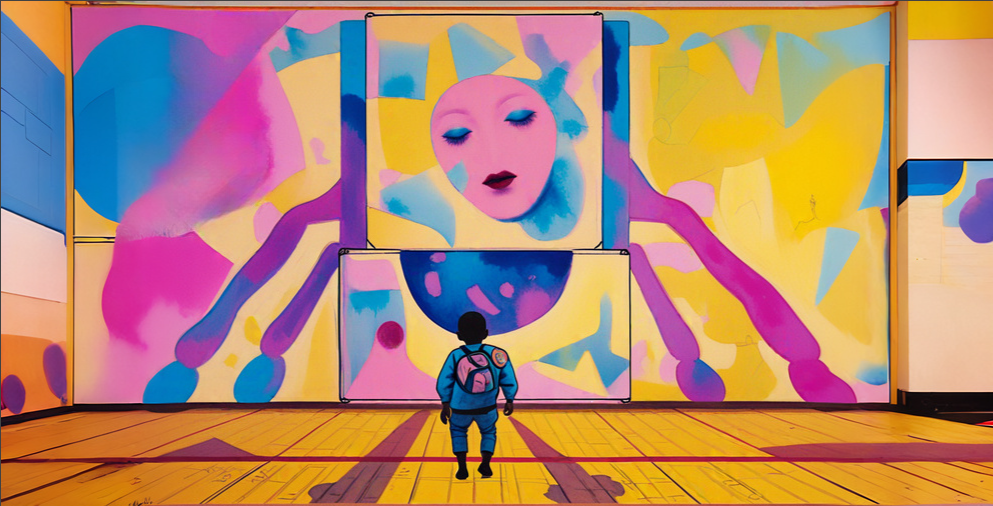
\includegraphics[width=\textwidth]{wBaordBanner.png}
    \caption{The spirit of the LLM WhiteBoard platform.}
    \vspace{0.1cm}
    \label{fig:spiritofWB}
\end{figure}

\subsection{Collaborative Paradigms in AI and HCI}

\subsubsection{Exploring Spatial and Semantic Interfaces}
The intersection of Human-Computer Interaction (HCI) and artificial intelligence has seen significant transformations with the advent of large language models (LLMs) acting as semantic operators.
These models bridge the gap between human intent and machine action, allowing users to interact with systems through high-level commands.
This paradigm enables more abstract, fluid interaction—users no longer need to micromanage interfaces but can instead provide overarching directives that the AI interprets and translates into executable code.
However, an equally important element in modern HCI design is the spatial aspect of collaboration, as seen in Spatial Pixel's work.
This combination of semantic understanding and spatial interaction is reshaping how we think about digital experiences.

\subsubsection{SpatialPixel and the Evolution of Digital Collaboration}
Traditional digital interfaces, largely confined to flat screens, often limit the user’s ability to engage with systems in meaningful ways.
This issue, sometimes referred to as "flat screen, flat thoughts,"\cite{whitney2024} highlights how modern interfaces—designed around two-dimensional layouts—can stifle creativity and limit interaction.
Violet Whitney and William Martin, through their work at Spatial Pixel, advocate for a more spatial approach to interface design.
They argue that human cognition is inherently spatial and embodied; our thoughts, behaviors, and problem-solving processes are deeply influenced by how we organize our physical environments.
In contrast to traditional screen-based systems, spatial interfaces allow users to leverage their embodied cognition, enhancing the possibilities for creative expression and complex problem solving.

SpatialPixel's work illustrates how knowledge work, much like manual labor, is inherently spatial.
Tools like Miro and Mural brought attention to this by allowing users to zoom out and organize tasks spatially on a canvas, mimicking how we naturally organize our workspaces in the physical world.
This concept of spatial cognition—the idea that we think through the space around us—provides an essential framework for the development of more immersive, AI-enhanced digital experiences.

\begin{figure}[!h]
    \centering
    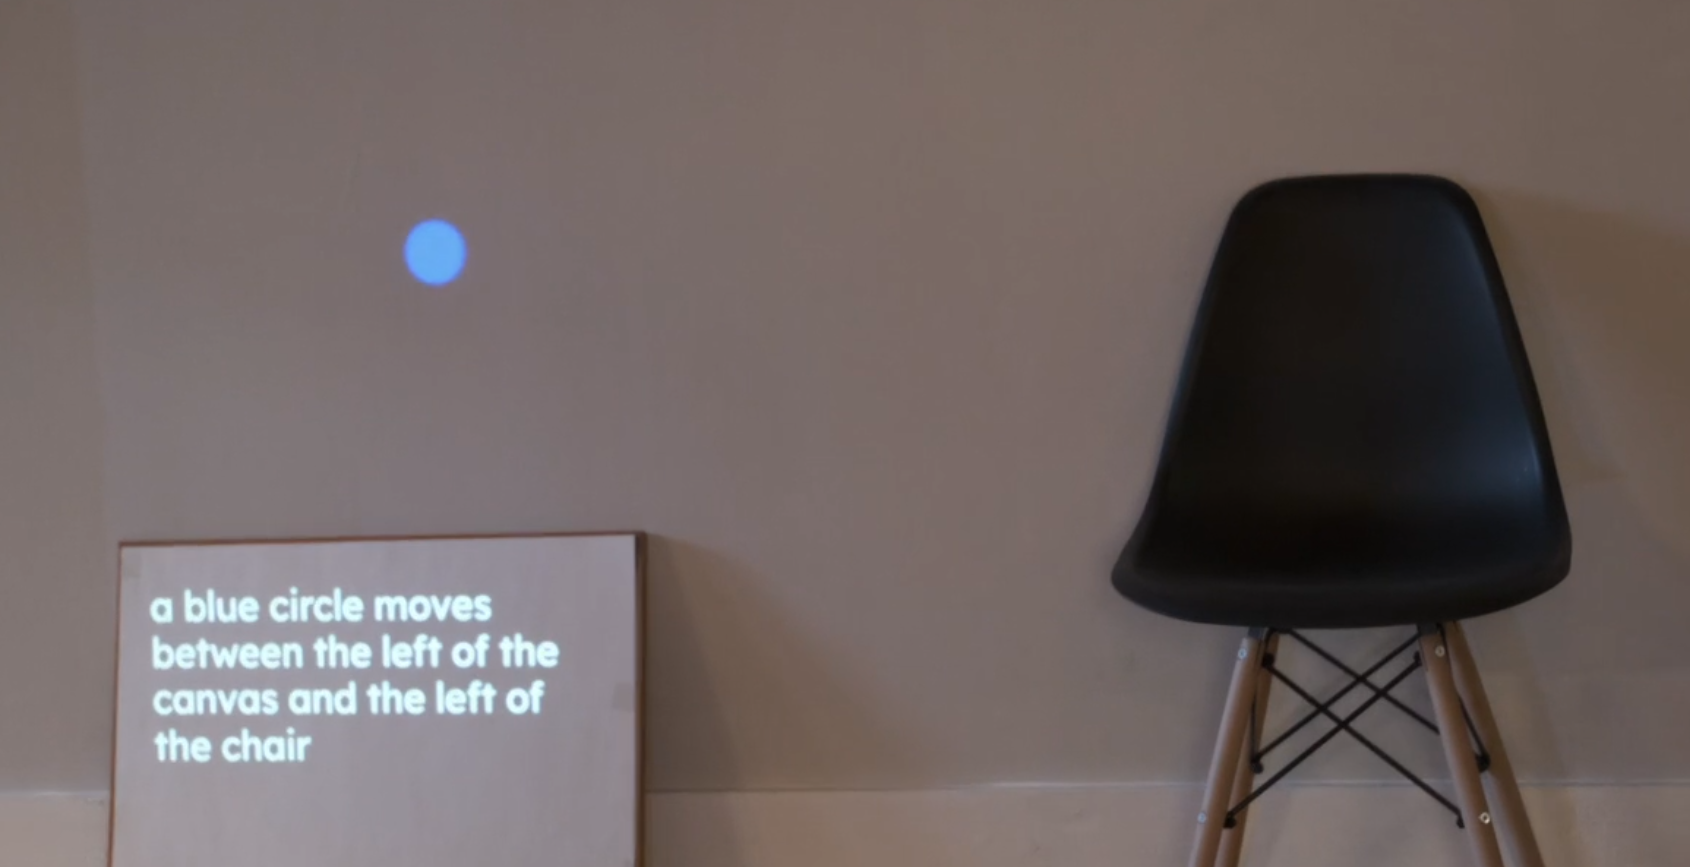
\includegraphics[width=\textwidth/3]{spatialpixel.png}
    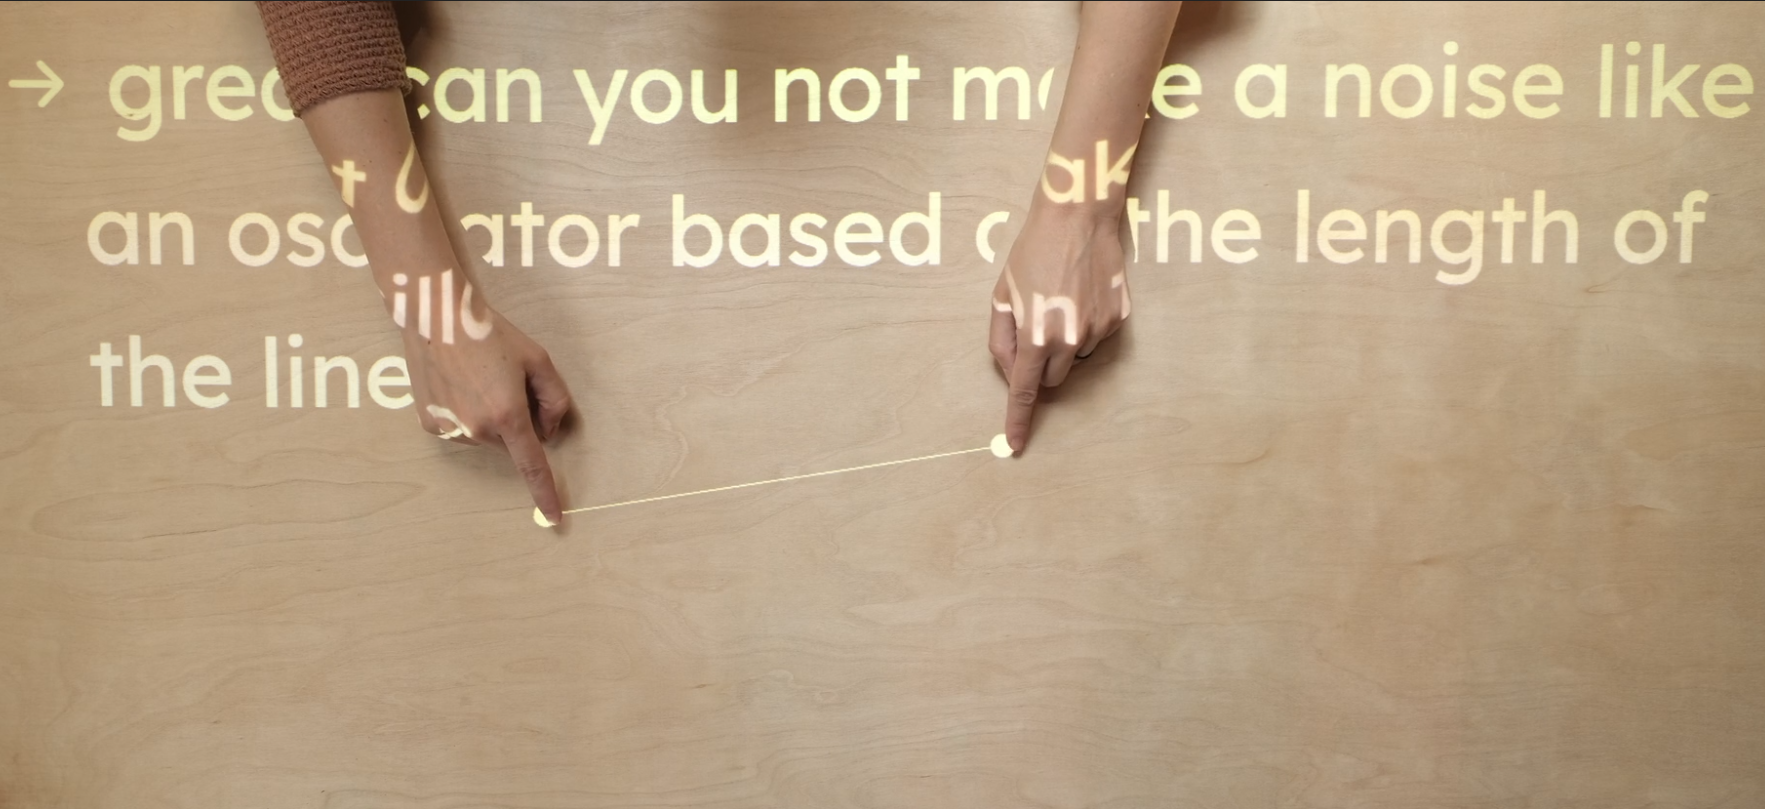
\includegraphics[width=\textwidth/3]{spatialpixel2.png}
    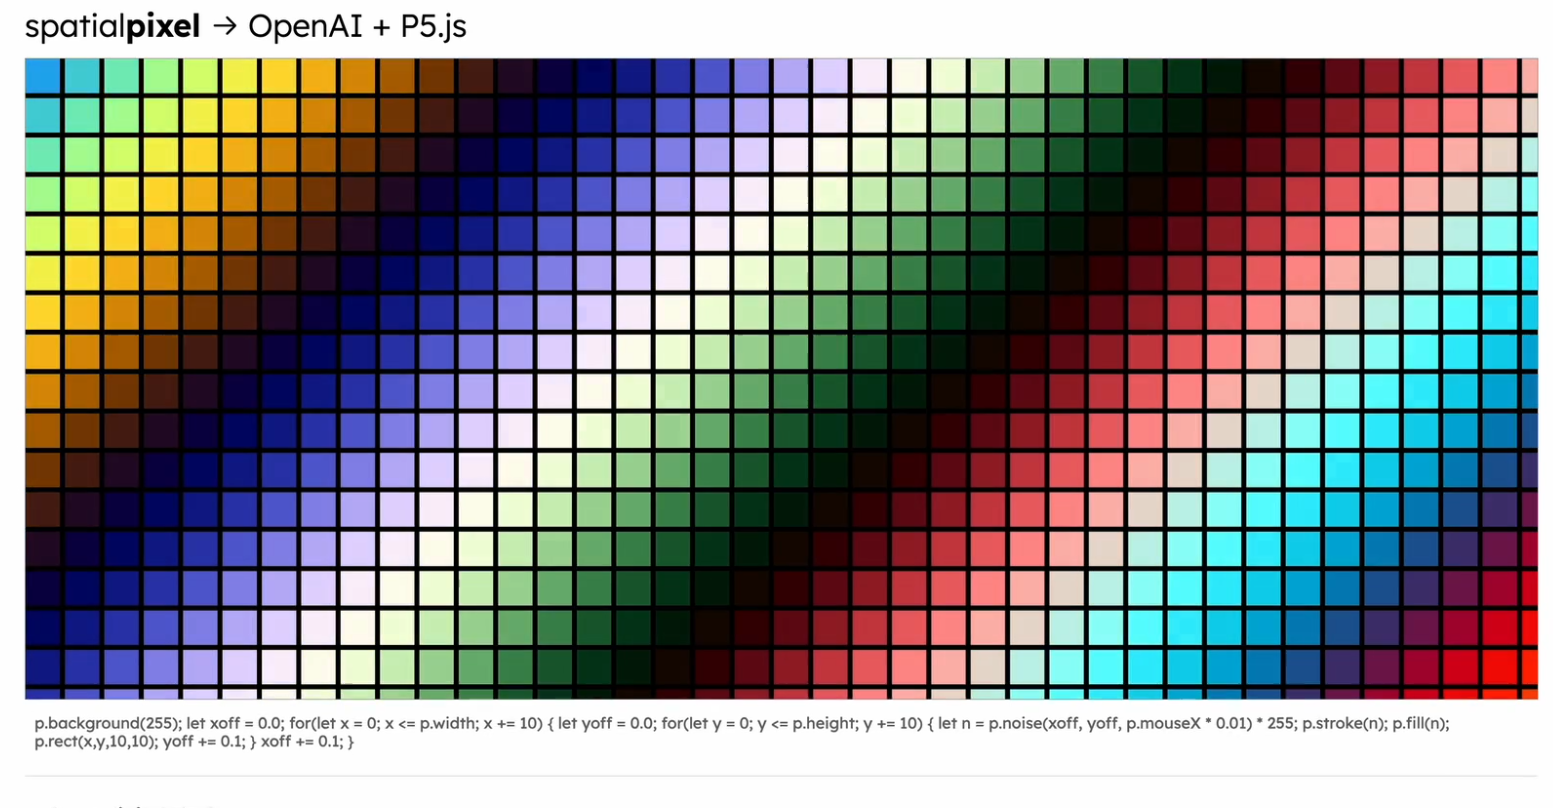
\includegraphics[width=\textwidth/3]{spatialpiwel3.png}
    \caption{Showcase of SpatialPixel's work on integrating spatial paradigms in LLM assisted applications.}
    \vspace{0.1cm}
    \label{fig:spatialpixel}
\end{figure}

The LLM Whiteboard project builds on these principles by combining the semantic power of LLMs with spatial interaction.
Users can issue commands to the LLM, which generates dynamic graphical elements within a p5.js environment.
This interaction becomes even more powerful when combined with spatial technologies, as demonstrated by the AR mode, where users can manipulate digital entities in real-world environments using Mediapipe.
Here, the spatial relationships between entities are not only visual but embodied, allowing users to interact with the system in ways that align with their natural cognitive processes.

For example, in the AR mode of the LLM Whiteboard, a user can point to a location within their physical environment, and the LLM, using Mediapipe, generates a corresponding digital entity in real-time. This interaction mimics how we naturally manipulate physical objects, further aligning the interface with the user’s cognitive expectations. By introducing spatiality into the interaction, the system enables a more intuitive and expansive form of collaboration, where both the LLM and the user co-create in a shared physical-digital space.


\subsubsection{Integrating LLMs with Spatial Intelligence}
By incorporating both semantic and spatial affordances, the LLM Whiteboard project creates a novel paradigm for collaborative digital interaction.
LLMs, as semantic operators, can handle high-level directives, translating abstract user inputs into specific actions.
At the same time, spatial technologies like Mediapipe allow for embodied interactions, grounding those digital actions in physical space.
This dual approach enables what can be described as low-signaling, high-possibility affordances—the system requires minimal input from the user to generate complex and meaningful outputs, while also allowing for expansive, freeform interactions that align with natural human cognition.

The integration of spatial computing further extends the collaborative possibilities by allowing users to offload cognitive tasks into the environment.
This aligns with the Extended Mind Theory, which suggests that cognitive processes are not confined to the brain but are distributed across the body and environment through the use of external tools.
LLMs, in this sense, serve as epistemic artifacts, tools that extend our ability to process information, while spatial interaction provides the physical grounding needed for effective problem-solving and creativity.


\subsection{The Role of Semantic Operators in AI-Driven Autonomy}
Large language models (LLMs) are increasingly acting as semantic operators—intelligent systems that bridge the gap between human intent and machine execution.
In this role, LLMs interpret high-level commands and autonomously generate corresponding actions, offering new possibilities for user interaction.
This shift from explicit command-based interactions to abstract, semantic-level collaboration represents a significant evolution in HCI, reducing the cognitive load on users while expanding their creative capabilities.

This section introduces key technologies, like Langchain\cite{chase2022}, that support the operation of LLMs as semantic operators, and integrates a discussion of current advancements in AI-driven autonomy, exemplified by AutoGPT\cite{autogpt2024}, BabyAGI\cite{nakajima2024}, and Microsoft Research’s “Sparks of Artificial General Intelligence” paper\cite{bubeck2023sparks}.
These developments collectively shape the way we understand how LLMs operate in complex digital systems, scaling their semantic capabilities and pushing toward broader, autonomous applications.

\subsubsection{LLMs as Semantic Operators}
At the core of the LLM Whiteboard project is the concept of LLMs functioning as semantic operators.
Rather than requiring explicit, low-level programming input, these models enable users to interact at a higher, more abstract level.
By processing human commands in natural language, LLMs act as intermediaries, translating user intent into executable actions or code.
This allows for the exploration of new forms of creative collaboration, where users are empowered to direct processes without the need for technical knowledge.

In this context, the concept of low-signaling, high-possibility affordances becomes central.
With minimal input from users—such as a simple command to "create a moving circle"—the LLM can generate complex, dynamic systems within a live coding environment.
Using technologies like p5.js for graphics and Langchain for tool orchestration, these models can handle complex digital tasks, manage the execution of various functions, and even self-correct through feedback loops.




\subsubsection{The Sea of LLM Agents: Scaling Semantic Capabilities}

As LLMs become more powerful, they evolve from standalone operators into distributed systems of LLM agents.
Each agent can specialize in different aspects of the task, collaborating with others to achieve higher complexity and scalability.
This concept of a sea of LLM agents, orchestrated through frameworks like Langchain, opens up vast possibilities for building autonomous systems that can perform tasks traditionally associated with human intelligence.

In the LLM Whiteboard project, this could involve multiple agents working in parallel—some handling the generation of graphical entities, others managing the interaction with external APIs, and yet another agent responsible for debugging and iterating on user feedback.
By decentralizing the task management process, the system becomes more flexible, scalable, and capable of handling complex workflows.

The emergence of autonomous multi-agent systems is emblematic of a broader trend in AI, as demonstrated by recent innovations like AutoGPT and BabyAGI.

\subsubsection{State of the Art: AutoGPT, BabyAGI, and Sparks of AGI}
The development of AutoGPT and BabyAGI offers a glimpse into how LLMs are being used as autonomous agents capable of handling complex tasks with minimal user input.
These systems represent the next step in scaling the semantic capabilities of LLMs, turning them into self-governing entities capable of multi-step reasoning, task decomposition, and even learning from experience.

\textbf{AutoGPT} demonstrates how LLMs can autonomously manage and complete tasks by breaking down high-level goals into subtasks and iterating over them without constant human guidance.
In a system like AutoGPT, LLMs go beyond responding to user prompts—they actively take on goals, strategize solutions, and execute actions autonomously.
This aligns with the goals of the LLM Whiteboard project, which seeks to minimize user input while maximizing creative output, allowing users to provide abstract commands that the model turns into executable code.

\textbf{BabyAGI} takes a learning-oriented approach to autonomy, focusing on task-oriented learning and recursive improvement.
This system simulates early stages of Artificial General Intelligence (AGI) by using feedback loops to iteratively improve its performance on tasks.
For the LLM Whiteboard, integrating BabyAGI-like capabilities would mean the system could learn from user interactions, refining its output based on real-time feedback.
This would enhance the model's ability to act as a creative partner, adapting to user preferences and improving its code generation over time.

\textbf{Sparks of AGI}, the paper published by Microsoft Research, explores the theoretical underpinnings of AGI, suggesting that LLMs are beginning to show early signs of general intelligence.
This research underlines the importance of multi-step reasoning and adaptability, features that are increasingly becoming part of systems like AutoGPT and BabyAGI.
The paper's insights reinforce the potential for LLMs to act as powerful semantic operators capable of handling complex, open-ended tasks that go beyond narrow use cases.

\subsubsection{Impact on the LLM Whiteboard Project}
The advances demonstrated by AutoGPT, BabyAGI, and the “Sparks of AGI” paper directly influence the trajectory of the LLM Whiteboard project.
As we integrate these cutting-edge concepts, we move toward a future where LLMs can serve as true creative collaborators, autonomously managing the complex digital experiences envisioned by users.
The incorporation of Langchain and the potential for multi-agent architectures allows the LLM Whiteboard to handle increasingly sophisticated design tasks with minimal intervention, reflecting the principles of low-signaling, high-possibility affordances in HCI.

By leveraging the operational power of autonomous agents, the LLM Whiteboard can expand its capabilities to include task learning, multi-agent collaboration, and iterative improvement.
This positions the project not just as a creative tool, but as a model for future systems that blend user-driven interaction with AI-driven autonomy, unlocking new possibilities for large-scale, adaptive digital experiences.

By incorporating the latest advances in AI-driven autonomy and task execution, the project demonstrates the profound potential of LLMs to act as powerful semantic operators—agents capable of transforming abstract user inputs into dynamic, creative outputs at scale.

\subsection{ Implementation of LLM Whiteboard}

The technical framework of the LLM Whiteboard revolves around two core technologies: Langchain and p5.js.

\subsubsection{Langchain: Operationalizing LLMs as Semantic Operators}

The technological backbone that empowers LLMs to operate as semantic agents within the LLM Whiteboard project is Langchain.
Acting both as a framework and an operational paradigm, Langchain orchestrates complex workflows by integrating LLMs with external tools and APIs, transforming them into tool-driven operators.
This allows the LLM to intelligently select the most appropriate resources for each task, making it more autonomous and responsive to user input.

In the LLM Whiteboard, Langchain enables the model to dynamically access and manipulate graphical entities in p5.js while simultaneously handling error correction and iteration.
For example, when the LLM is asked to "create a bouncing ball," it generates the required code in p5.js, while managing the visual attributes and behaviors of the entity in real time.
This seamless interaction between user commands and the model's code generation capabilities is made possible by Langchain's orchestration logic.

\begin{figure}[h!]
    \centering
    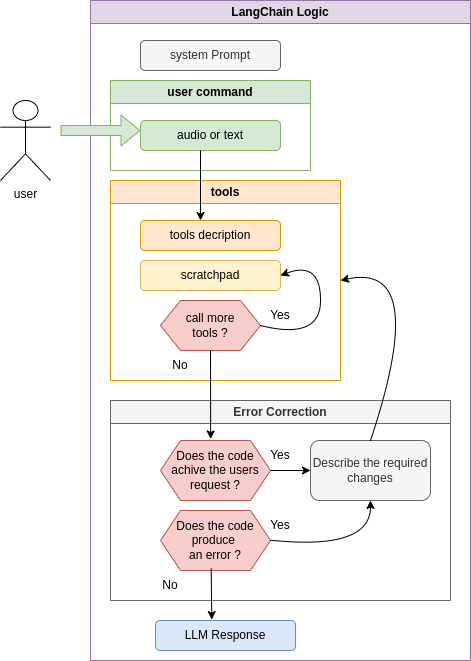
\includegraphics[width=\textwidth/2]{errorCL.drawio.png}
    \caption{Diagram of the LangChain Logic used for error correction.}
    \vspace{0.1cm}
    \label{fig:langchainlogic}
\end{figure}

Langchain’s architecture supports zero-shot prompting, allowing the model to generate new entities and functions on the fly by accessing predefined tools and APIs.
Furthermore, Langchain enables a robust fallback mechanism that empowers the model to correct and iterate on its code autonomously. Beyond its specific application in the LLM Whiteboard, Langchain lays the groundwork for scaling LLM-based systems into more sophisticated autonomous agents, capable of handling complex, multi-domain tasks.

\subsubsection{p5.js : The Seeds of Creative Coding}

\textbf{p5.js} is an open-source JavaScript library created by \textbf{Lauren McCarthy} in 2014, inspired by the Processing language developed by Casey Reas and Ben Fry.
Its main goal is to simplify coding through an accessible and playful approach, using gamification to make programming more engaging.
By offering real-time visual feedback, p5.js encourages experimentation, making coding less intimidating, especially for beginners.

More than just a learning tool, p5.js enables a new art form that integrates visuals, audio, and interaction.
It allows artists to create dynamic, generative works that respond to user inputs, blending technology and creativity in ways that redefine digital art.
p5.js supports a global creative community, fostering inclusivity and accessibility in creative coding while expanding the possibilities for interactive art and multimedia experiences.

\subsubsection{System Architecture}

p5.js provides the graphical environment where the LLM Whiteboard brings user commands to life.
The LLM uses this library to instantiate and manipulate entities like circles, rectangles, or more complex forms, linking abstract user inputs to visual outputs.
p5.js’s ability to handle real-time animations and dynamic user interactions makes it an ideal platform for this form of AI-assisted creation.
Additionally, the LLM can extend p5.js's core functionality by writing custom functions that augment the library’s capabilities, further expanding the creative space available to the user.

\begin{figure}[h!]
    \centering
    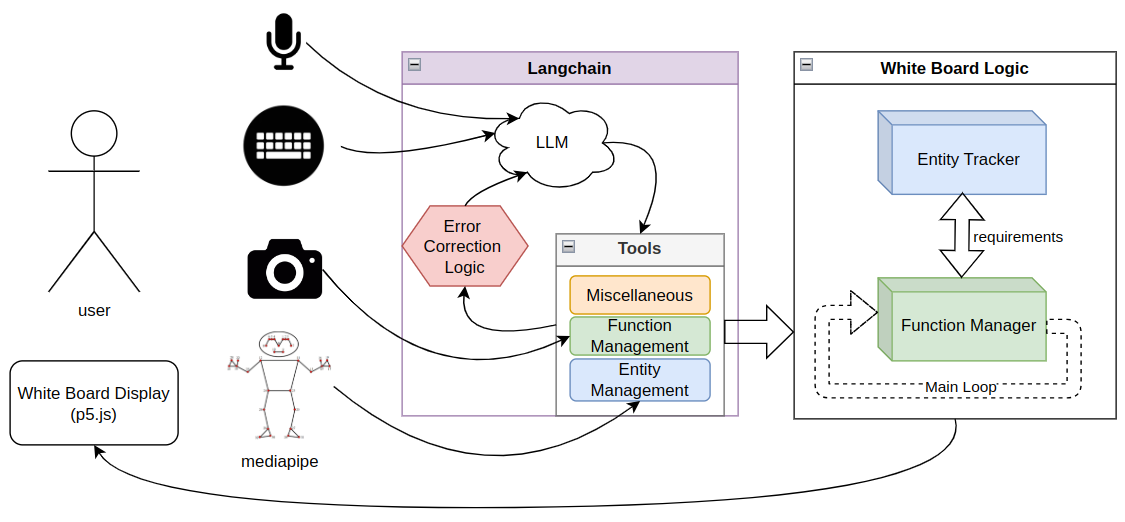
\includegraphics[width=\textwidth]{llmwhiteboard.drawio.png}
    \caption{Architecture diagram of the LLM WhiteBoard.}
    \vspace{0.1cm}
    \label{fig:wbarchietcure}
\end{figure}

The LLM White Board offers multiple modalities of interaction, enhancing the user’s ability to engage with both the creative and technical aspects of the system.
Commands can be sent via keyboard or voice, allowing users to express their high-level ideas in a flexible manner.
Interaction with the generated creations is facilitated through either the mouse or Mediapipe, enabling intuitive control over digital entities.
Additionally, a drop-down menu provides access to the code associated with the entities and functions created by the LLM, offering users a deeper understanding of the system’s underlying processes and actions.

\begin{figure}[h!]
    \centering
    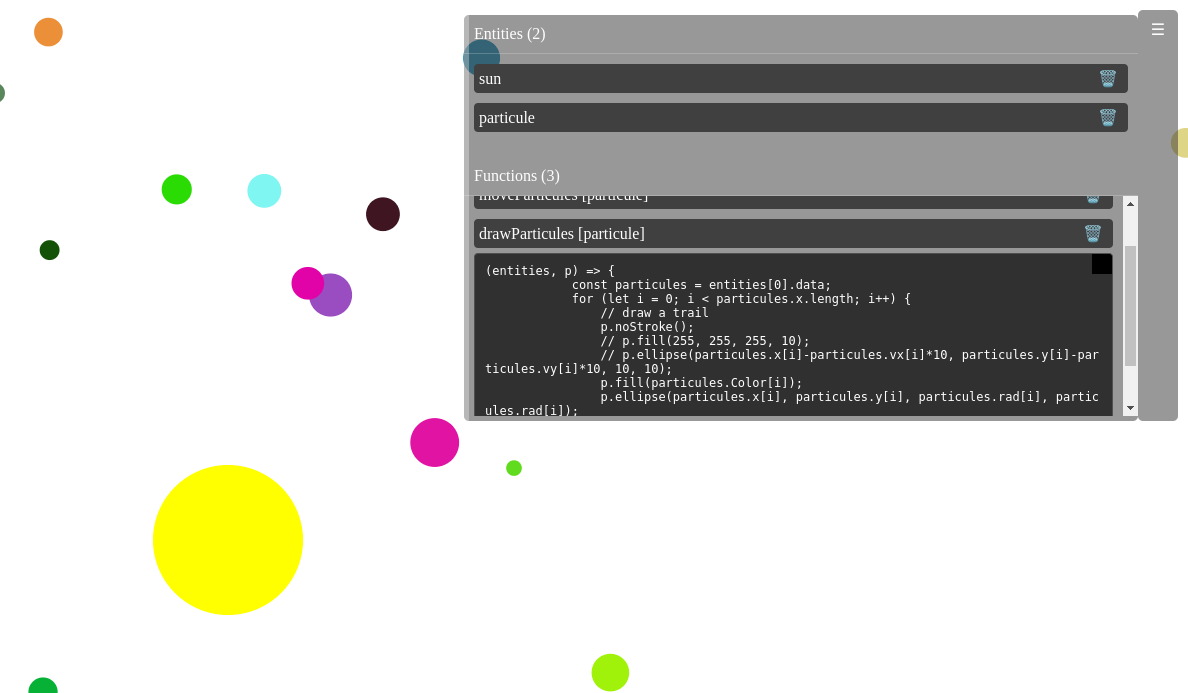
\includegraphics[width=\textwidth]{wbmenu.png}
    \caption{Menu allowing user to see the code generated by the LLM.}
    \vspace{0.1cm}
    \label{fig:wbmenu}
\end{figure}

Together, these technologies form the foundation of a system that combines user-driven creativity with the autonomous problem-solving abilities of LLMs.
The LLM Whiteboard thus stands as a demonstration of how AI can enable new forms of interaction in HCI, allowing users to explore high-possibility, low-signaling affordances that lower the barrier to creative expression while expanding the range of what can be accomplished with minimal input.

\subsubsection{Modes of Interaction}

1. \textbf{In White Board mode}: the canvas starts as a blank space, and the collaboration between the user and the LLM is visually displayed on top of the canvas.
This mode emphasizes a dynamic, fluid interaction, where the LLM generates code in real time based on high-level instructions from the user.
Whether via text or voice input, the user can issue commands such as "create a circle" or "generate a wave pattern," and the LLM translates these into the corresponding p5.js code.

The affordance here lies in the way the system abstracts the technical complexity behind coding.
Rather than requiring the user to understand the intricate syntax of JavaScript or p5.js, the system transforms abstract ideas into executable functions.
This not only accelerates the creative process but also lowers the barrier for non-technical users to engage in coding-based design.
The error correction mechanism, enabled by Langchain, further enhances the experience by providing immediate feedback and iterating over solutions when errors arise, ensuring smooth and uninterrupted interaction.

\begin{figure}[h!]
    \centering
    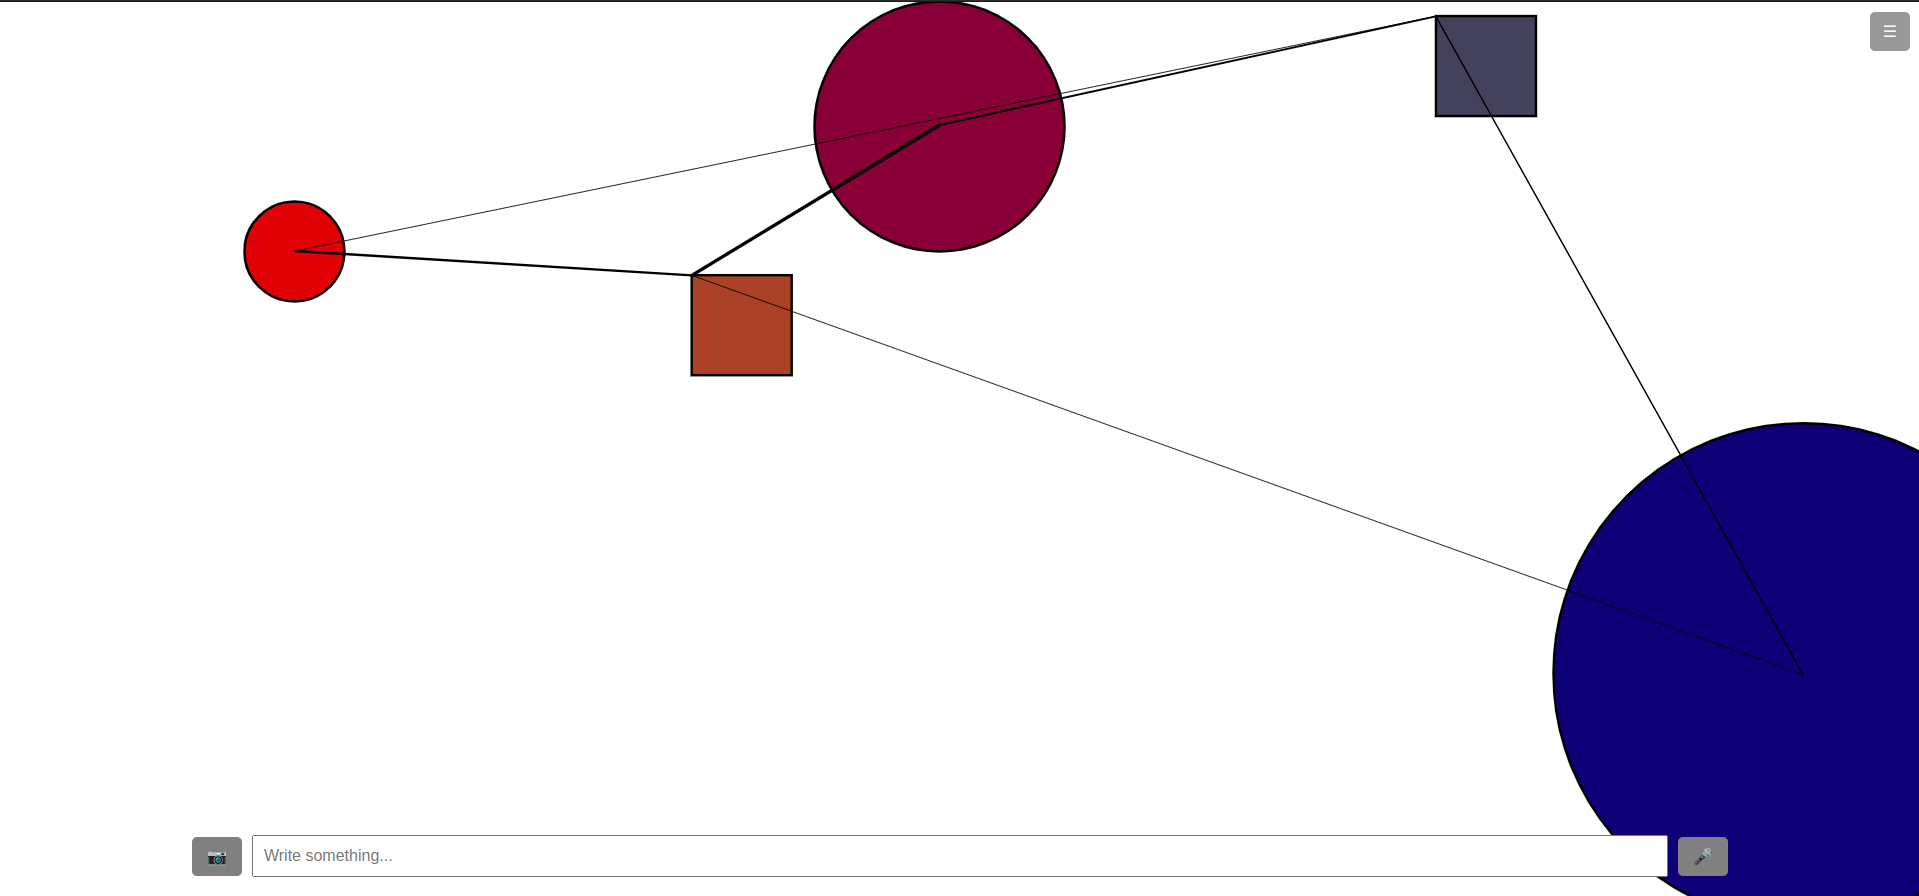
\includegraphics[width=\textwidth/3]{wbexp1.png}
    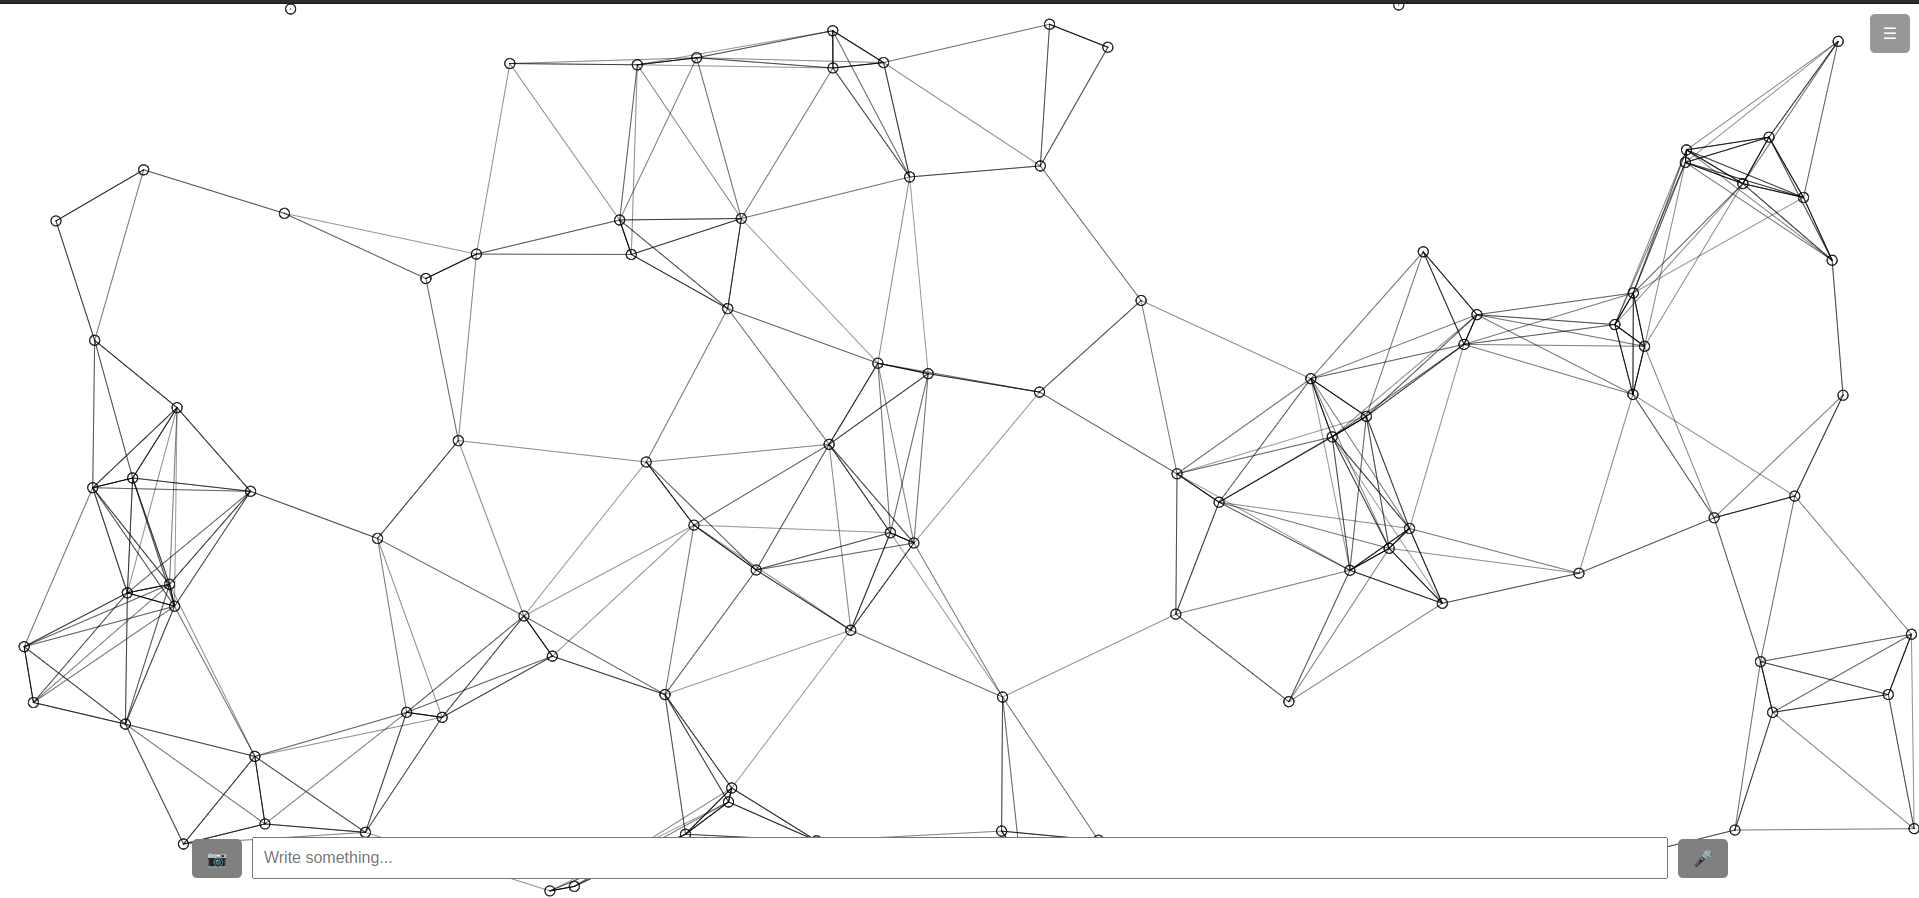
\includegraphics[width=\textwidth/3]{wbexp2.png}
    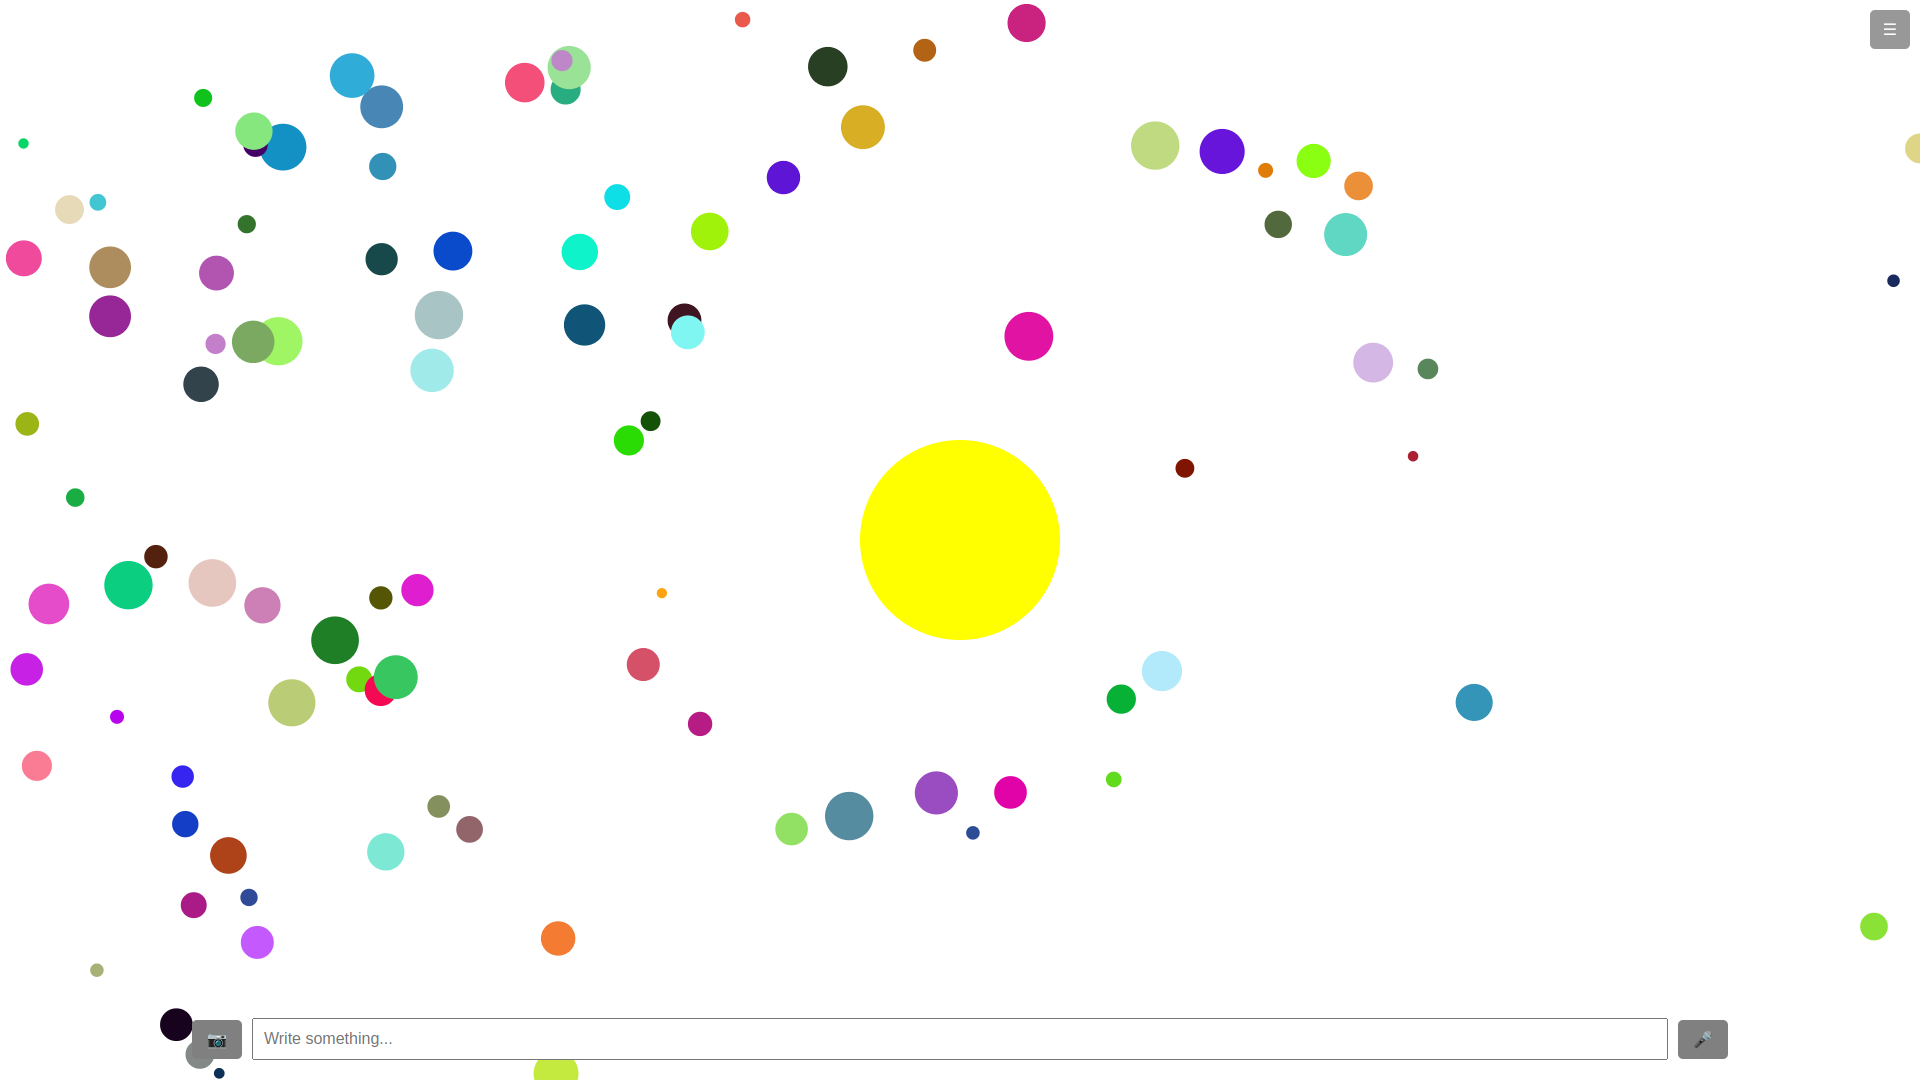
\includegraphics[width=\textwidth/3]{wbexp3.png}
    \caption{Demonstration of the LLM WhiteBoard in action.}
    \vspace{0.1cm}
    \label{fig:wbdemo1}
\end{figure}

2. \textbf{AR mode:} The second mode extends the interaction possibilities by introducing the physical world into the equation.
In this mode, the user’s webcam feed is overlaid onto the canvas, creating a mixed-reality environment where both digital and physical elements coexist.
Through the integration of Mediapipe, the LLM is able to track the user’s body, hands, and face, allowing it to create entities and functions that respond to the user’s movements.

For example, the LLM can be prompted to generate functions that change the color of an object based on hand gestures or move an entity in response to body position.
This interactivity adds a new layer of immersion and control, as the user's physical presence becomes an integral part of the digital creation process.
The affordances in this mode are defined by the system’s ability to bridge the gap between digital interaction and physical movement, creating a seamless blend of AR and AI-driven functionality.

The use of AR in combination with AI allows for high-level creative experimentation that would traditionally require intricate knowledge of both computer vision and real-time interaction systems.
Here again, the system simplifies the complex technical aspects, such as mediating between body tracking inputs and code execution, into a set of high-level commands that the LLM can interpret and act upon.
This transforms the experience into one where the user’s natural gestures and movements become creative tools, opening up a wide range of possibilities for interactive digital experiences.

\begin{figure}[h!]
    \centering
    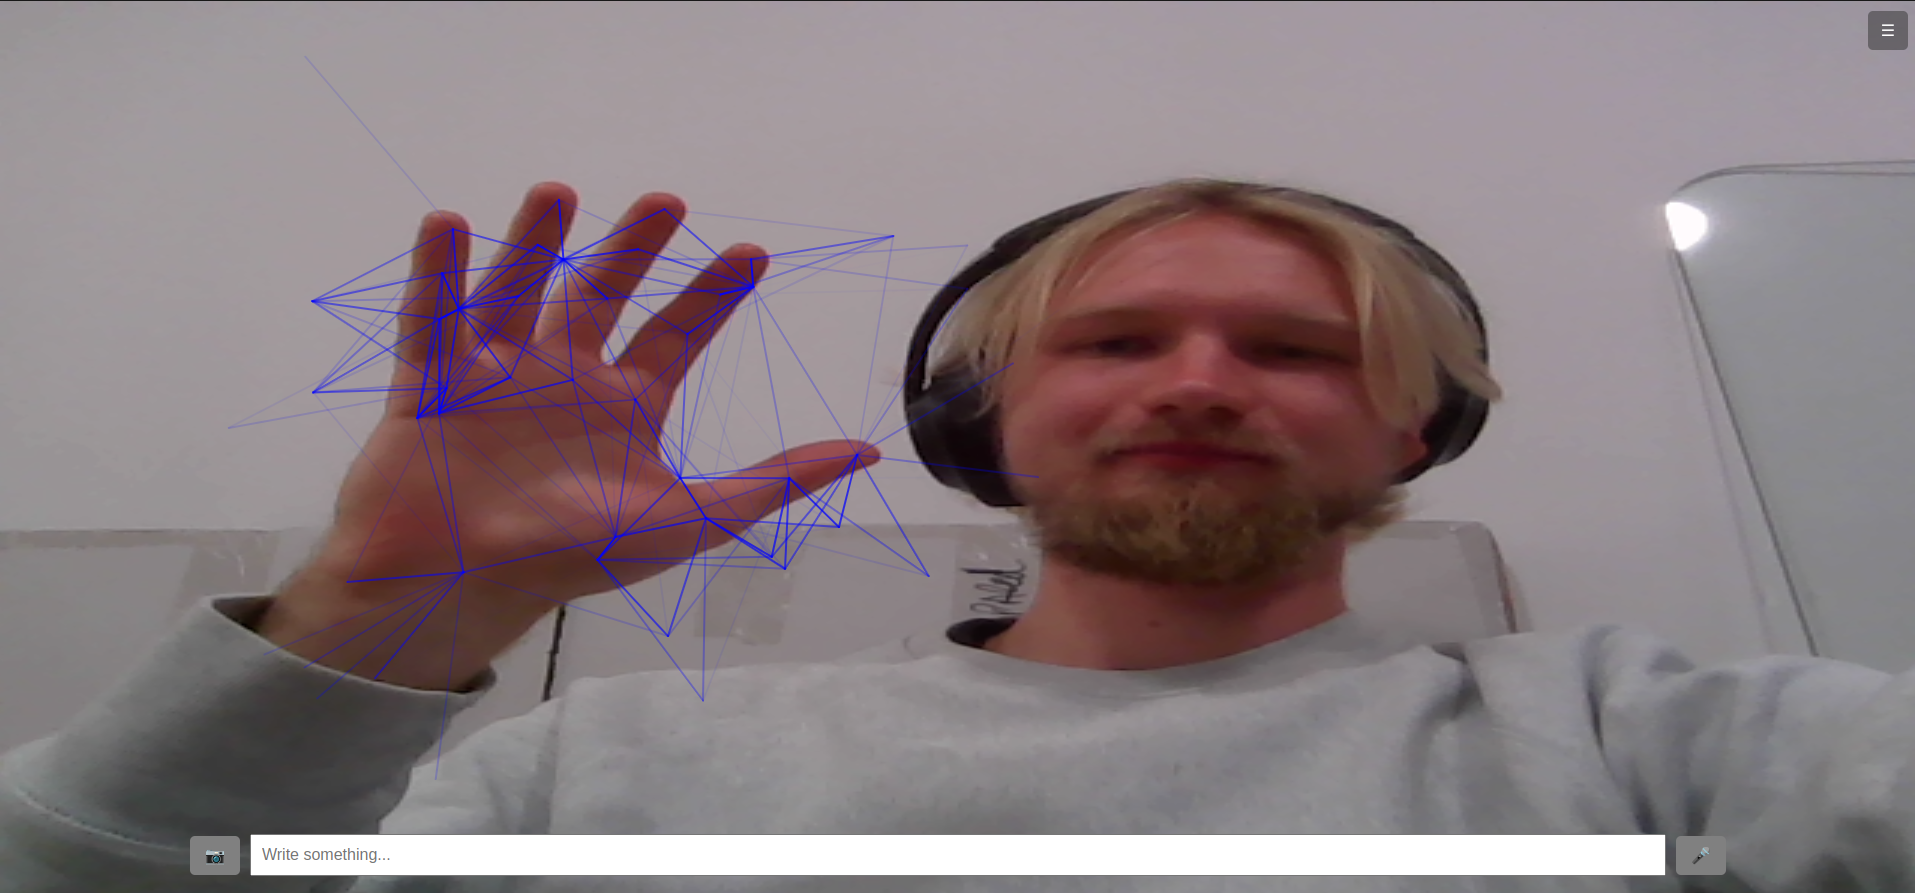
\includegraphics[width=\textwidth/3]{wbexpar1.png}
    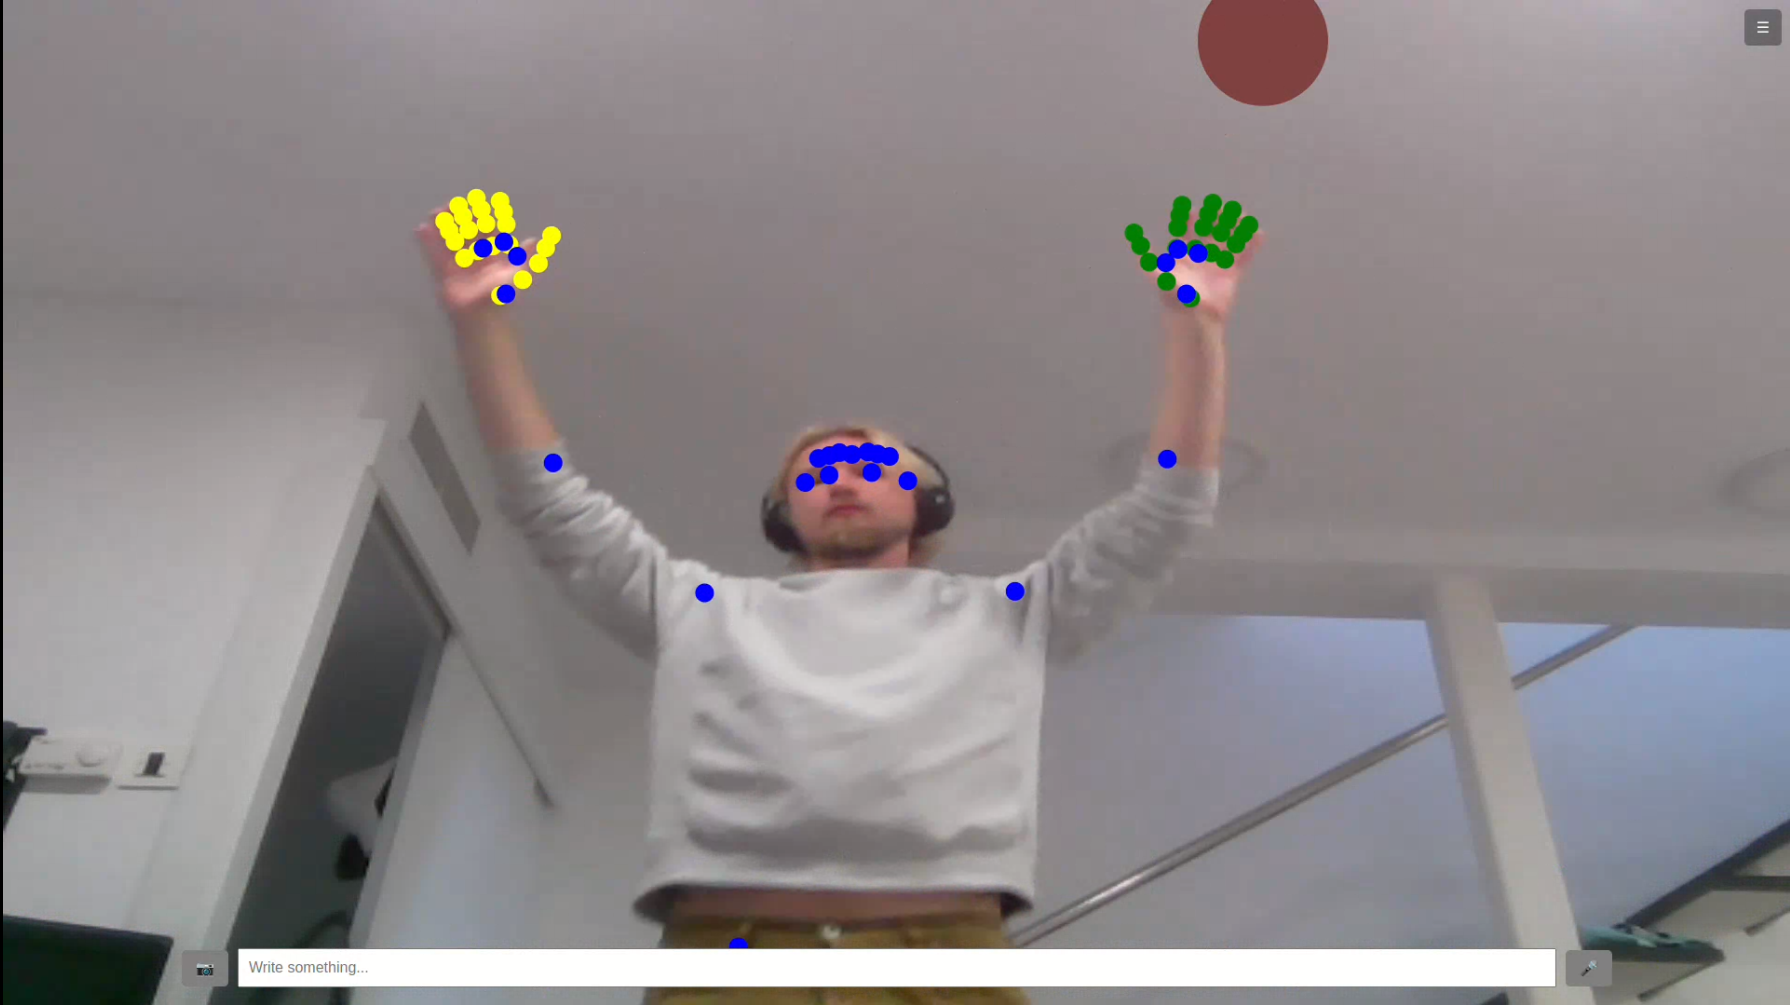
\includegraphics[width=\textwidth/3]{wbexpar2.png}
    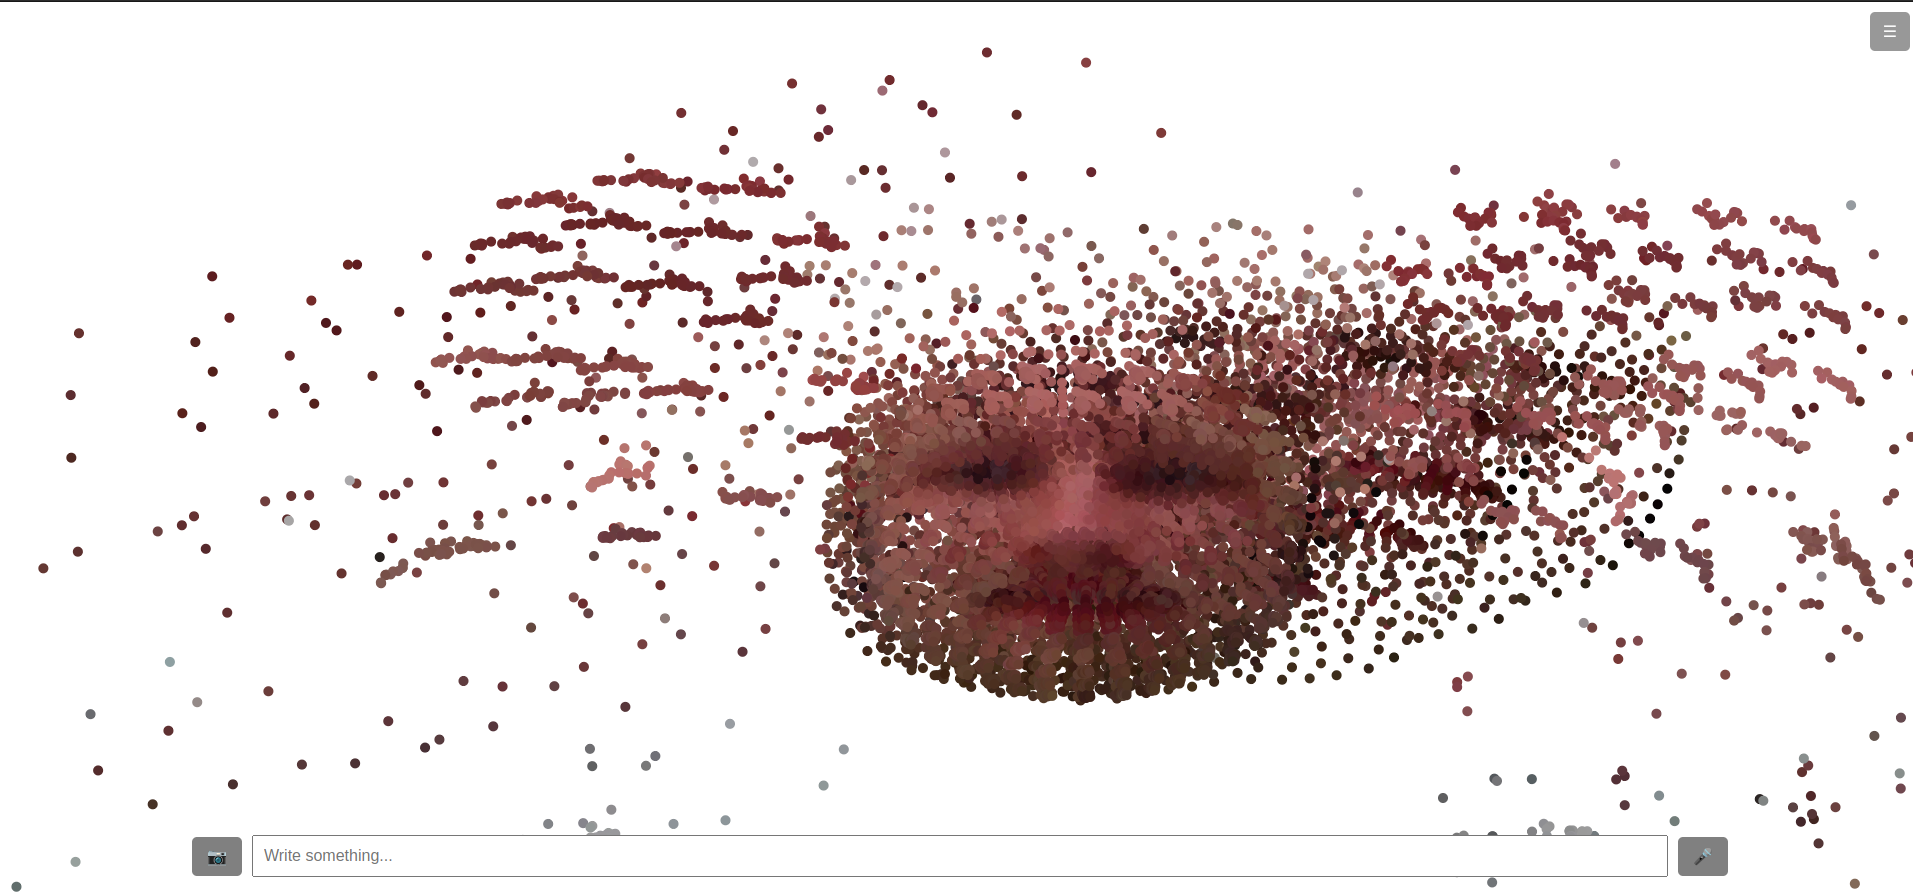
\includegraphics[width=\textwidth/3]{wbexpar3.png}
    \caption{Demonstration of the AR mode of the LLM WhiteBoard in action.}
    \vspace{0.1cm}
    \label{fig:wbdemo1}
\end{figure}

\subsection{Conclusion}

The \textbf{LLM Whiteboard} project demonstrates how the integration of LLMs and spatial interaction technologies can redefine the creative process within Human-Computer Interaction.
By leveraging LLMs as semantic operators, the platform transforms high-level user commands into executable code in a live coding environment.
This allows users to interact with digital creations more intuitively, minimizing the technical complexity typically involved in coding-based systems.

The system’s dual modalities—White Board and AR—offer two distinct forms of interaction.
In White Board mode, users can issue commands that generate dynamic entities and functions in p5.js, all within a visual, real-time canvas.
Meanwhile, in AR mode, the physical environment is incorporated, allowing users to interact with digital objects through natural movements and gestures, tracked via Mediapipe.

At its core, the LLM Whiteboard reduces the barrier for entry into digital creation, making it more accessible to non-technical users while also enabling rapid prototyping and collaboration.
By fusing the abstract capabilities of LLMs with spatial computing, the platform opens up new avenues for interactive digital experiences.

\subsubsection{Discussion}

The LLM Whiteboard project sparks discussions regarding the evolving role of AI in creative processes and HCI.
First, it highlights the potential for LLMs to act as creative collaborators rather than mere tools.
By interpreting high-level inputs and generating complex outputs autonomously, these models take on more creative responsibility, prompting the question: how much of the creative process can or should be handed over to AI?

Another crucial discussion point is the merging of spatial and semantic interfaces.
As the platform demonstrates, spatial interactions—enabled by AR and body tracking—provide a more natural and embodied way for users to engage with digital content.
This aligns with cognitive theories, such as the Extended Mind Theory, which suggest that cognition is distributed between the brain, body, and environment.
The LLM Whiteboard’s ability to extend digital creation into physical space offers a glimpse into how future systems might further integrate human cognition with AI-driven environments.

The system also raises questions about accessibility.
By abstracting away the complexities of coding, it makes creative coding environments more inclusive, allowing a wider range of users to explore digital design without needing in-depth technical knowledge.
This democratization of tools is a key trend in modern HCI and has significant implications for the future of creative technology.

\subsubsection{Final Thoughts}

The \textbf{LLM Whiteboard} project stands at the intersection of AI and spatial computing, offering a powerful glimpse into the future of creative collaboration in HCI.
By using LLMs to handle the semantic layer and spatial technologies to enable natural interaction, the platform makes digital creation more intuitive, accessible, and engaging.
The two modes—White Board and AR—offer flexible pathways for users to explore their creative ideas, whether through abstract commands or physical gestures.

In doing so, the LLM Whiteboard not only reduces the technical barriers to digital creativity but also expands the possibilities for interaction.
It bridges the gap between human intent and machine execution, showcasing how AI can become a true creative partner in the digital realm.
The project sets a foundation for future innovations where LLMs and spatial intelligence combine to create even more immersive, adaptive, and user-driven digital experiences.
